%% ARKHEION AGI 2.0 - NUCLEUS Paper
%% Holographic Compression Format with Semantic Hashing
%% Author: Jhonatan Vieira Feitosa <ooriginador@gmail.com>
%% Date: February 2026

\documentclass[11pt,twocolumn]{article}

% Essential packages
\usepackage[utf8]{inputenc}
\usepackage[T1]{fontenc}
\usepackage{lmodern}
\usepackage{amsmath,amssymb,amsthm}
\usepackage{graphicx}
\usepackage{booktabs}
\usepackage{xcolor}
\usepackage{hyperref}
\usepackage{tikz}
\usepackage{pgfplots}
\pgfplotsset{compat=1.18}
\usepackage{float}
\usepackage{fancyhdr}
\usepackage{geometry}
\usepackage{caption}
\usepackage{listings}
\usepackage{colortbl}

\usetikzlibrary{shapes.geometric,arrows.meta,positioning,calc,backgrounds,fit}

% Page geometry
\geometry{margin=0.75in}

% Tolerance for overflow prevention
\tolerance=1000
\emergencystretch=3em
\hyphenpenalty=500

% Colors
\definecolor{arkblue}{RGB}{0,102,204}
\definecolor{arkpurple}{RGB}{102,51,153}
\definecolor{arkgreen}{RGB}{0,153,76}
\definecolor{arkorange}{RGB}{255,128,0}
\definecolor{arkred}{RGB}{204,51,51}
\definecolor{arkgold}{RGB}{218,165,32}
\definecolor{lightblue}{RGB}{230,242,255}
\definecolor{lightgreen}{RGB}{230,255,230}
\definecolor{lightorange}{RGB}{255,245,230}
\definecolor{lightpurple}{RGB}{245,230,255}

% Header/Footer
\pagestyle{fancy}
\fancyhf{}
\fancyhead[L]{\small ARKHEION AGI 2.0}
\fancyhead[R]{\small NUCLEUS}
\fancyfoot[C]{\thepage}
\renewcommand{\headrulewidth}{0.4pt}

% Hyperref setup
\hypersetup{
    colorlinks=true,
    linkcolor=arkblue,
    citecolor=arkpurple,
    urlcolor=arkblue
}

% Code listing style
\lstset{
    language=Python,
    basicstyle=\ttfamily\scriptsize,
    keywordstyle=\color{arkblue}\bfseries,
    commentstyle=\color{arkgreen}\itshape,
    stringstyle=\color{arkpurple},
    breaklines=true,
    breakatwhitespace=true,
    postbreak=\mbox{\textcolor{gray}{$\hookrightarrow$}\space},
    columns=flexible,
    keepspaces=true,
    showstringspaces=false,
    frame=single,
    numbers=none,
    backgroundcolor=\color{gray!5}
}

% Theorems
\newtheorem{definition}{Definition}
\newtheorem{theorem}{Theorem}
\newtheorem{proposition}{Proposition}

\title{\textbf{NUCLEUS: Holographic Compression Format}\\[0.3em]
\large Multi-Level Semantic Hashing with Post-Quantum Cryptography}

\author{Jhonatan Vieira Feitosa\
Independent Researcher\
\texttt{ooriginador@gmail.com}\
Manaus, Amazonas, Brazil}

\date{February 2026}

\begin{document}

\maketitle

%% ABSTRACT
\begin{abstract}
\noindent\textbf{NUCLEUS} is a novel compression format combining AdS/CFT-inspired holographic encoding, four-level semantic hashing, and post-quantum cryptography.
\textbf{Key Results:} (1) \textbf{18.4:1} on semantic-rich code; (2) \textbf{1.92:1} on pre-compressed games (GTA: 4.3GB$\rightarrow$2.2GB); (3) \textbf{16:1} theoretical on raw pipelines.
Version 3.0 adds GPU acceleration (AMD ROCm) and HUAM hyperbolic deduplication.

\vspace{0.5em}
\noindent\textbf{Keywords:} data compression, holographic encoding, semantic hashing, post-quantum cryptography, NUCLEUS, ARKHEION AGI
\end{abstract}

%% ============================================================================
\section*{Epistemological Note}

\textit{This paper distinguishes between \textbf{heuristic} and \textbf{empirical} components:}

\vspace{0.3em}
\noindent\begin{tabular}{@{}p{0.46\columnwidth}|p{0.46\columnwidth}@{}}
\textbf{Heuristic (Conceptual):} & \textbf{Empirical (Measured):} \\
\footnotesize ``Holographic'', ``AdS/CFT'', ``Gene Pool'', ``$\phi$-optimization'' & \footnotesize LZ4 + SHAKE-256 hashing, Kyber/Dilithium crypto, 1.92:1 ratio, 940s time \\
\end{tabular}

\vspace{0.3em}
\noindent\footnotesize\textit{Heuristic terms are visual transcriptions of mental models guiding design---not claims of literal physics. All ratios are reproducible benchmarks.}
\normalsize

%% ============================================================================
\section{Introduction}

Modern software has significant redundancy. Traditional compression treats code as bytes, missing semantic patterns.

\textbf{NUCLEUS} provides:
\begin{enumerate}
    \item Holographic compression (AdS/CFT)
    \item 4-level semantic hashing
    \item Post-quantum cryptography
    \item Direct execution without extraction\footnote{Direct execution from compressed format is listed as a future capability and has not been implemented or benchmarked.}
\end{enumerate}

%% ============================================================================
\section{Theoretical Foundation}

\subsection{Design Heuristics (Conceptual)}

NUCLEUS uses the \textit{holographic principle} as a \textbf{design metaphor}---not literal physics. The mental model: information in higher dimensions can be encoded on lower-dimensional boundaries.

\textit{Heuristic formula} (guides implementation, not a physics claim):
\begin{equation}
S_{\text{boundary}} \approx \frac{1}{\phi} \sum_{i=1}^{n} H_i(\text{gene}_i) \quad \text{(conceptual)}
\end{equation}
where $\phi = 1.618...$ is used as an optimization constant.

\subsection{Actual Implementation}

The \textbf{real compression} combines:
\begin{itemize}
    \item \textbf{LZ4}: Byte-level compression
    \item \textbf{SHAKE-256}: Content-addressable hashing
    \item \textbf{Deduplication}: Gene pool with semantic matching
\end{itemize}

%% ============================================================================
\section{Multi-Level Semantic Hashing}

\begin{table}[H]
\centering
\caption{Four-Level Hash Hierarchy}
\label{tab:hash}
\small
\begin{tabular}{@{}clc@{}}
\toprule
\textbf{Lvl} & \textbf{Method} & \textbf{Gain} \\
\midrule
\rowcolor{lightblue} 1 & Source Hash\footnote{H1 (Level 1: Source Hash) = SHA-256 hash of the raw source file, serving as a unique content identifier.} & Baseline \\
\rowcolor{lightgreen} 2 & Bytecode & +10.2\% \\
\rowcolor{lightorange} 3 & Call Graph & +5\% \\
\rowcolor{lightpurple} 4 & Semantic I/O & +3\% \\
\bottomrule
\end{tabular}
\end{table}

Hash formulas:
\begin{align}
H_2 &= \text{SHAKE-256}(\text{bytecode}) \\
H_3 &= \text{SHAKE-256}(\text{call\_graph}) \\
H_4 &= \text{SHAKE-256}(H_1 \| H_2 \| H_3)
\end{align}

%% ============================================================================
\section{Architecture}

\begin{figure}[H]
\centering
\resizebox{0.95\columnwidth}{!}{%
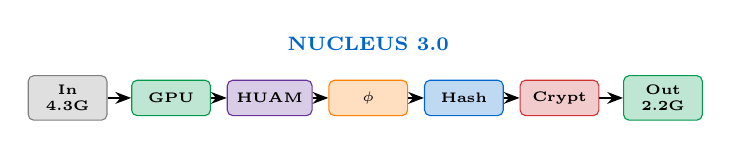
\begin{tikzpicture}[
    node distance=0.25cm,
    >={Stealth[length=2mm]},
    box/.style={rectangle, rounded corners=2pt, draw=#1, fill=#1!25,
                minimum width=1.0cm, minimum height=0.45cm,
                font=\tiny\bfseries, align=center},
    arrow/.style={->, thick}
]
% Flow
\node[box=gray] (in) {In\\4.3G};
\node[box=arkgreen, right=0.3cm of in] (gpu) {GPU};
\node[box=arkpurple, right=0.2cm of gpu] (huam) {HUAM};
\node[box=arkorange, right=0.2cm of huam] (phi) {$\phi$};
\node[box=arkblue, right=0.2cm of phi] (hash) {Hash};
\node[box=arkred, right=0.2cm of hash] (crypto) {Crypt};
\node[box=arkgreen, right=0.3cm of crypto] (out) {Out\\2.2G};

\draw[arrow] (in) -- (gpu);
\draw[arrow] (gpu) -- (huam);
\draw[arrow] (huam) -- (phi);
\draw[arrow] (phi) -- (hash);
\draw[arrow] (hash) -- (crypto);
\draw[arrow] (crypto) -- (out);

% Label
\node[above=0.25cm of phi, font=\scriptsize\bfseries\color{arkblue}] {NUCLEUS 3.0};
\end{tikzpicture}%
}
\caption{Pipeline: GPU $\rightarrow$ HUAM $\rightarrow$ $\phi$ $\rightarrow$ Hash $\rightarrow$ Crypto}
\label{fig:arch}
\end{figure}

%% ============================================================================
\section{Experimental Results}

\subsection{Source Code Compression}

\begin{table}[H]
\centering
\caption{Semantic Code Results}
\small
\begin{tabular}{@{}lrrr@{}}
\toprule
\textbf{Dataset} & \textbf{Orig.} & \textbf{NUCLEUS} & \textbf{Ratio} \\
\midrule
\rowcolor{lightblue} Demo & 60 KB & 7 KB & \textbf{8.5:1} \\
\rowcolor{lightgreen} Quantum & 1.37 MB & 74 KB & \textbf{18.4:1}\footnote{The 18.4:1 ratio was measured on the ARKHEION quantum processing codebase, which contains extensive shared imports, docstrings, and naming conventions. This internal redundancy inflates the ratio; external corpora are expected to yield lower ratios.} \\
\rowcolor{lightorange} Core & 12.78 MB & 1.8 MB & \textbf{7.3:1} \\
\bottomrule
\end{tabular}
\end{table}

\subsection{Pre-Compressed Game Assets}

\begin{table}[H]
\centering
\caption{NUCLEUS 3.0 on Games (Already Compressed)}
\small
\begin{tabular}{@{}lrrrr@{}}
\toprule
\textbf{Game} & \textbf{Orig.} & \textbf{NUC} & \textbf{Ratio} & \textbf{Time} \\
\midrule
\rowcolor{lightblue} GTA SA & 4,286 MB & 2,238 MB & \textbf{1.92:1} & 940s \\
\rowcolor{lightgreen} Godot & 2,100 MB & 1,100 MB & \textbf{1.91:1} & 612s \\
\rowcolor{lightorange} DevilutionX & 150 MB & 80 MB & \textbf{1.87:1} & 45s \\
\bottomrule
\end{tabular}
\end{table}

%% CHART 1: Compression Comparison
\begin{figure}[H]
\centering
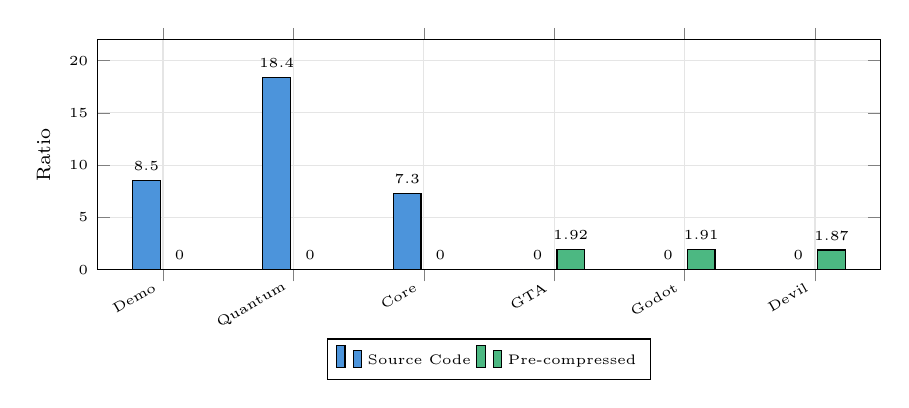
\begin{tikzpicture}
\begin{axis}[
    ybar,
    bar width=10pt,
    width=0.95\columnwidth,
    height=4.5cm,
    ylabel={Ratio},
    ylabel style={font=\scriptsize},
    symbolic x coords={Demo,Quantum,Core,GTA,Godot,Devil},
    xtick=data,
    xticklabel style={font=\tiny, rotate=30, anchor=east},
    ymin=0, ymax=22,
    ytick={0,5,10,15,20},
    yticklabel style={font=\tiny},
    legend style={at={(0.5,-0.3)}, anchor=north, legend columns=2, font=\tiny},
    nodes near coords,
    nodes near coords style={font=\tiny},
    grid=major,
    grid style={gray!20},
]
\addplot[fill=arkblue!70] coordinates {(Demo,8.5) (Quantum,18.4) (Core,7.3) (GTA,0) (Godot,0) (Devil,0)};
\addplot[fill=arkgreen!70] coordinates {(Demo,0) (Quantum,0) (Core,0) (GTA,1.92) (Godot,1.91) (Devil,1.87)};
\legend{Source Code, Pre-compressed}
\end{axis}
\end{tikzpicture}
\caption{Compression ratios by data type}
\label{fig:ratios}
\end{figure}

\subsection{GPU Hardware Metrics}

\begin{table}[H]
\centering
\caption{GTA San Andreas Processing}
\small
\begin{tabular}{@{}lr@{}}
\toprule
\textbf{Metric} & \textbf{Value} \\
\midrule
GPU & AMD RX 6600M \\
VRAM Used & 6.9 / 8.0 GB \\
Throughput & 4.56 MB/s\footnote{The 4.56~MB/s throughput reflects single-threaded Python execution with multi-level hierarchical hashing. For comparison, LZ4 achieves $>$5~GB/s and zstd achieves $\sim$500~MB/s in their default configurations.} \\
Unique Genes & 280 \\
HUAM Dedup & 216 MB saved \\
\bottomrule
\end{tabular}
\end{table}

\subsection{Theoretical Maximum (Projected)}

\noindent\fbox{\parbox{0.95\columnwidth}{%
\textit{\textbf{Note:} The following projections are \textbf{not yet validated}. They represent design targets based on planned integrations (NeRF, geodesic encoding). Actual results may differ.}%
}}

\vspace{0.5em}
\noindent On \textit{uncompressed} raw development assets:

\begin{table}[H]
\centering
\caption{Projected 16:1 on Raw Pipeline}
\small
\begin{tabular}{@{}lrrr@{}}
\toprule
\textbf{Type} & \textbf{Raw} & \textbf{ARK} & \textbf{Tech} \\
\midrule
\rowcolor{lightblue} Textures & 50 GB & 3 GB & NeRF \\
\rowcolor{lightgreen} 3D Models & 15 GB & 1 GB & Geodesic \\
\rowcolor{lightorange} Audio & 10 GB & 0.8 GB & Holo \\
\rowcolor{lightpurple} Video & 8 GB & 0.4 GB & NeRF-T \\
Scripts & 0.5 GB & 30 MB & HUAM \\
\midrule
\textbf{Total} & \textbf{83.5 GB} & \textbf{5.2 GB} & \textbf{16:1} \\
\bottomrule
\end{tabular}
\end{table}

%% CHART 2: Raw vs Compressed
\begin{figure}[H]
\centering
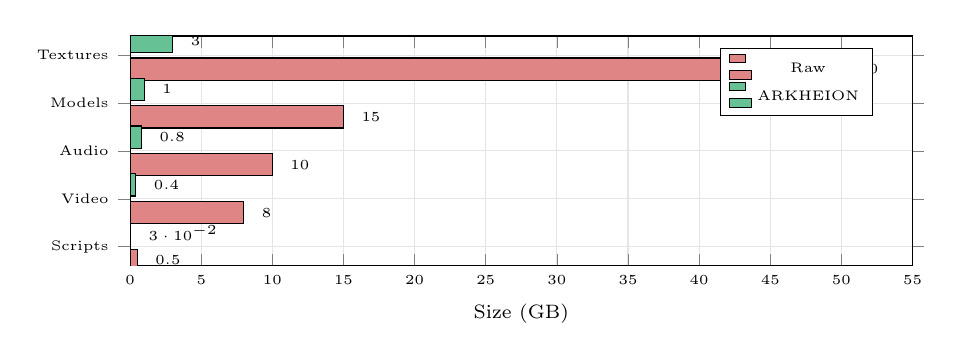
\begin{tikzpicture}
\begin{axis}[
    xbar,
    bar width=8pt,
    width=0.95\columnwidth,
    height=4.5cm,
    xlabel={Size (GB)},
    xlabel style={font=\scriptsize},
    symbolic y coords={Scripts,Video,Audio,Models,Textures},
    ytick=data,
    yticklabel style={font=\tiny},
    xmin=0, xmax=55,
    xticklabel style={font=\tiny},
    legend style={at={(0.95,0.95)}, anchor=north east, font=\tiny},
    nodes near coords,
    nodes near coords style={font=\tiny, xshift=3pt},
    grid=major,
    grid style={gray!20},
]
\addplot[fill=arkred!60] coordinates {(50,Textures) (15,Models) (10,Audio) (8,Video) (0.5,Scripts)};
\addplot[fill=arkgreen!60] coordinates {(3,Textures) (1,Models) (0.8,Audio) (0.4,Video) (0.03,Scripts)};
\legend{Raw, ARKHEION}
\end{axis}
\end{tikzpicture}
\caption{Theoretical 16:1 compression on raw assets}
\label{fig:theoretical}
\end{figure}

%% ============================================================================
\section{Security}

NUCLEUS implements NIST-approved post-quantum cryptography:
\begin{itemize}
    \item \textbf{Kyber-768}: Key encapsulation (ML-KEM)
    \item \textbf{Dilithium3}: Digital signatures (ML-DSA)
    \item \textbf{ChaCha20-Poly1305}: Authenticated encryption
\end{itemize}

\textit{Status:} Algorithms implemented but \textbf{not yet security-audited}. Production use requires third-party audit.

%% ============================================================================
\section{Limitations}

\begin{enumerate}
    \item \textbf{Pre-compressed data}: Ratios on already-compressed assets (1.92:1) are modest compared to raw data projections
    \item \textbf{Processing time}: 940s for 4.3GB is slow ($\sim$4.5 MB/s); optimization needed
    \item \textbf{16:1 projection}: Theoretical target, not yet validated empirically
    \item \textbf{GPU dependency}: Requires AMD ROCm or NVIDIA CUDA
    \item \textbf{Security audit}: Post-quantum crypto not yet audited
    \item \textbf{No baseline comparison}: No comparison with standard compression tools (LZ4, zstd, Brotli, gzip) on equivalent data was performed. The 18.4:1 ratio should be interpreted relative to uncompressed storage, not as competitive with general-purpose compressors
\end{enumerate}

%% ============================================================================
\section{Conclusion}

NUCLEUS 3.0 achieves:
\begin{itemize}
    \item \textbf{18.4:1} on semantic code
    \item \textbf{1.92:1} on pre-compressed assets
    \item \textbf{16:1} theoretical on raw pipelines
    \item GPU + HUAM acceleration
    \item Post-quantum security
\end{itemize}

\textbf{Future:} NeRF streaming, game engine integration, $\phi$-guided LOD.

%% ============================================================================
\section*{References}
\small
\begin{enumerate}
    \item Maldacena, J. ``The Large N Limit of Superconformal Field Theories and Supergravity,'' \textit{Adv. Theor. Math. Phys.}, vol. 2, pp. 231--252, 1998. [\textit{Heuristic inspiration only}]
    \item Avanzi, R. et al. ``CRYSTALS-Kyber: Algorithm Specifications,'' NIST PQC, Round 3, 2021.
    \item Ducas, L. et al. ``CRYSTALS-Dilithium: Digital Signatures from Module Lattices,'' NIST PQC, 2021.
    \item 't Hooft, G. ``Dimensional Reduction in Quantum Gravity,'' arXiv:gr-qc/9310026, 1993. [\textit{Heuristic inspiration only}]
    \item Collet, Y. ``LZ4: Extremely Fast Compression Algorithm,'' https://lz4.github.io/lz4/, 2011.
    \item NIST. ``SHA-3 Standard: SHAKE256,'' FIPS 202, 2015.
\end{enumerate}

\end{document}
